\subsection{Sentiment Prediction for ConceptNet}
Random walk is commonly used to spread values on a graph~\cite{Wu:relSelect14,Hassan:ACL10,Xu:COLING10,Cambria:AAAI10}. It spreads values through synonym and antonym edges. The equation of random walk with restart is as follows:
\begin{equation}
\label{eq:rndWalk}
\boldsymbol{s}_{t+1} = (1-\alpha)\boldsymbol{W}\boldsymbol{s}_t + \alpha\boldsymbol{s}_0
\end{equation}
where $\boldsymbol{s}_t$ is the values of each node when the $t$-th iteration. $\boldsymbol{W}$ is a similarity matrix, which can be acquired from sources like Ontology, ConceptNet, corpus, etc. Similarity matrix of a standard random walk is an out-link normalized matrix. $\alpha$ is the restarting weight. Random walk is an iterative process, and after $n$ iteration, each node spreads its value to the neighbors that are $n$ links distant from it.

In previous research~\cite{Tsai:IEEE13, Wu:relSelect14}, random walk is applied to propagate values on ConceptNet. They found that in ConceptNet, performing in-link normalized on similarity matrix is better than performing out-link normalized because out-link normalization will underestimate the influence of concepts with more neighbors. In in-link normalization, each concept's new sentiment value in the ($t+1$)-th iteration is the average of all its neighbors in the $t$-th iteration.

\subsection{Latent Dirichlet Allocation}
Latent Dirichlet Allocation (LDA)~\cite{Blei:LDA03} is a generative probabilistic model of a corpus, in which documents are represented as random mixtures over latent topics, and each topic is characterized by a distribution over words. The intuition behind LDA is that each document exhibits multiple topics. It exploits word co-occurrence information to capture latent topics in the corpus.

In LDA, each document $d$ is represented by bag of words (so the order of words in a document is not considered), and each document is assumed to be generated by the following (given parameters of Dirichlet distribution $\boldsymbol{\alpha}$ and per-topic word distribution $\boldsymbol{\beta}$):
\begin{enumerate}[]
	\item Choose probability coefficients over topics $\boldsymbol{\theta}_d {\sim} Dir(\boldsymbol{\alpha})$
	\item For each of the $N$ word positions $x_{d,n}$:
	\begin{enumerate}
		\item Choose a topic assignment $z_{d,n} {\sim} Multinomial(\boldsymbol{\theta})$
		\item Choose a word $w_{d,n}$ conditioned on the chosen topic $z_{d,n}$ and the per-topic word distribution $\boldsymbol{\beta}_{z_{d,n}}$
	\end{enumerate}
\end{enumerate}

From the generative process, the graphical model representation of basic LDA is shown in Figure~\ref{fig:LDA_model}. Observing word co-occurrence in each document, LDA infers topic probability coefficients $\boldsymbol{\theta}_d$ for each document and topic assignment $z_{d,n}$ for each word of each document to maximize the likelihood of this corpus. However, the posterior distribution is intractable for exact inference of each $\boldsymbol{theta}_d$ and $z_{d,n}$. Blei {\it et al.} use variational EM to infer these latent variables and find parameters $\boldsymbol{\alpha}$ and $\boldsymbol{\beta}$ to maximize the log likelihood of given corpus.

\begin{figure}[!t]
\centering
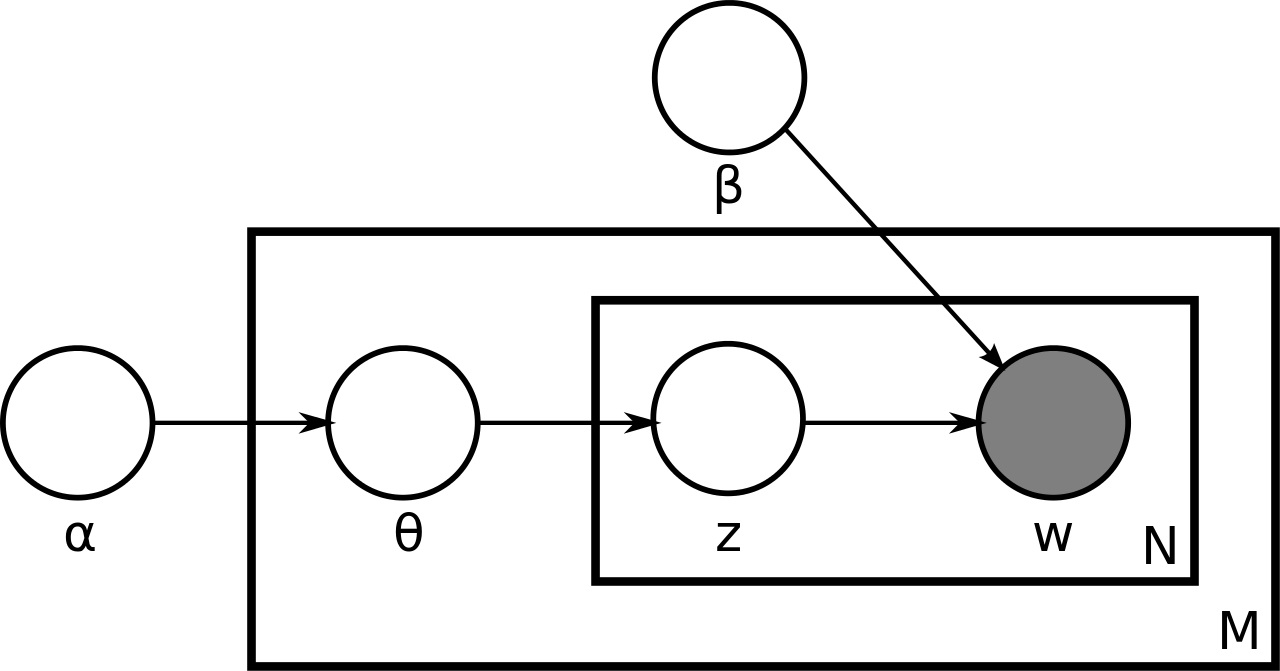
\includegraphics[width=2.5in]{fig/LDA_model.jpg}
\caption{Graphical model representation of LDA.}
\label{fig:LDA_model}
\end{figure}

Because the words coverage for each document is sparse, they smooth multinomial parameters $\boldsymbol{\beta}$ by generating $\boldsymbol{\beta}_k \sim Dir(\boldsymbol{\eta})$ for each topic, shown in Figure~\ref{fig:LDA_model2}. They infer $\boldsymbol{\beta}_k$ by modify the variational model, like inferring $\boldsymbol{\theta}_d$.

\begin{figure}[!t]
\centering
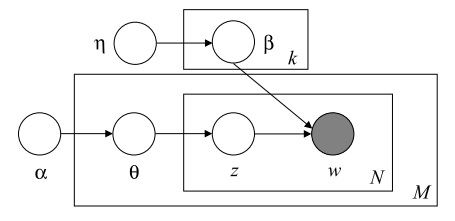
\includegraphics[width=2.5in]{fig/LDA_model2.jpg}
\caption{Graphical model representation of smoothed LDA.}
\label{fig:LDA_model2}
\end{figure}

As the result, LDA infers $\boldsymbol{\theta}_d$ for each document, $z_{d,n}$ for each word of document and $\boldsymbol{\beta}_k$ for each topic. Besides, it estimates $\boldsymbol{\alpha}$ and $\boldsymbol{\eta}$ as the model of this corpus.